\documentclass[fleqn,answers,addpoints]{exam}

%\usepackage{graphicx, fancyhdr}
\usepackage{etoolbox}
\usepackage{subcaption}
\usepackage{etoolbox}
\usepackage{tikz,pgfplots}
\usepackage{amsmath, amsfonts}
\usepackage{color}

%% For LaTeX-Box: root = stat105_exam1_info.tex 
%%%%%%%%%%%%%%%%%%%%%%%%%%%%%%%%%%%%%%%%%%%%%%%%%%%%%%%%%%%%%%%%%%%%%%%%%%%%%%%%
%  File Name: stat105_exam1_info.tex
%  Purpose:
%
%  Creation Date: 24-09-2015
%  Last Modified: Thu Sep 24 13:51:36 2015
%  Created By:
%%%%%%%%%%%%%%%%%%%%%%%%%%%%%%%%%%%%%%%%%%%%%%%%%%%%%%%%%%%%%%%%%%%%%%%%%%%%%%%%
\newcommand{\course}[1]{\ifstrempty{#1}{STAT 105}{STAT 105, Section #1}}
\newcommand{\sectionNumber}{B}
\newcommand{\examDate}{October 1, 2015}
\newcommand{\semester}{FALL 2015}
\newcommand{\examNumber}{II}

\newcommand{\examTitle}{Exam \examNumber}

\runningheader{\course{\sectionNumber}}{Exam \examNumber}{\examDate}
\runningfooter{}{}{Page \thepage of \numpages}

\newcommand{\examCoverPage}{
   \begin{coverpages}
   \centering
   {\bfseries\scshape\Huge Exam I \par}
   \vspace{1cm}
   {\bfseries\scshape\LARGE \course{\sectionNumber} \par}
   {\bfseries\scshape\LARGE \semester \par}

   \vspace{2cm}

   \fbox{\fbox{\parbox{5.5in}{\centering 

      \vspace{.25cm} 
      
      {\bfseries\Large Instructions} \\

      \vspace{.5cm} 

      \begin{itemize}
         \item  The exam is scheduled for 80 minutes, from 8:00 to 9:20 AM. At 9:20 AM the exam will end.\\
         \item  A forumula sheet is attached to the end of the exam. Feel free to tear it off.\\
         \item  You may use a calculator during this exam.\\
         \item  Answer the questions in the space provided. If you run out of room, continue on the back of the page. \\
         \item  If you have any questions about, or need clarification on the meaning of an item on this exam, please ask your instructor. No other form of external help is permitted attempting to receive help or provide help to others will be considered cheating.\\
         \item  {\bfseries Do not cheat on this exam.} Academic integrity demands an honest and fair testing environment. Cheating will not be tolerated and will result in an immediate score of 0 on the exam and an incident report will be submitted to the dean's office.\\
      \end{itemize}

   }}}

   \vspace{2cm}

   \makebox[0.6\textwidth]{Name:\enspace\hrulefill}

   \vspace{1cm}

   \makebox[0.6\textwidth]{Student ID:\enspace\hrulefill}
   \end{coverpages}

}


\newcommand{\course}[1]{\ifstrempty{#1}{STAT 305}{STAT 305, Section #1}}
\newcommand{\sectionNumber}{}
\newcommand{\examDate}{May 8, 2019}
\newcommand{\semester}{Spring 2019}
\newcommand{\examNumber}{3}
\newcommand{\qparts}[1]{\begin{parts} #1 \end{parts}}
\newcommand{\qitems}[1]{\begin{itemize} #1 \end{itemize}}

% Document definitions
\newcommand{\examTitle}{Exam \examNumber}
\runningheader{\course{\sectionNumber}}{Exam \examNumber}{\examDate}
\runningfooter{}{}{Page\ \thepage\ of\ \numpages}

\begin{document}

\begin{coverpages}
   \centering
   {\bfseries\scshape\Huge Exam \examNumber \par}
   \vspace{1cm}
   {\bfseries\scshape\LARGE \course{\sectionNumber} \par}
   {\bfseries\scshape\LARGE \semester \par}
   \vspace{2cm}
   \fbox{\fbox{\parbox{5.5in}{
      \centering 
      \vspace{.25cm} 
      {\bfseries\Large Instructions} \\
      \vspace{.25cm} 
      \begin{itemize}
         \item  The exam is scheduled for 120 minutes, from 12:00 to 2:00pm. At  2:00pm  the exam will end.\\
         \item  A forumula sheet is attached to the end of the exam. Feel free to tear it off.\\
         \item  You are allowed to use a self-produced one-page (front and back) formula sheet during this exam.\\
         \item  You may use a calculator during this exam.\\
         \item  Answer the questions in the space provided. If you run out of room, continue on the back of the page. \\
         \item  If you have any questions about, or need clarification on the meaning of an item on this exam, please ask your instructor. No other form of external help is permitted attempting to receive help or provide help to others will be considered cheating.\\
         \item  {\bfseries Do not cheat on this exam.} Academic integrity demands an honest and fair testing environment. Cheating will not be tolerated and will result in an immediate score of 0 on the exam and an incident report will be submitted to the office of the dean.\\
      \end{itemize}
   }}}
   \vspace{1cm}
   \makebox[0.6\textwidth]{}
   \vspace{1cm}
   \makebox[0.6\textwidth]{Name:\enspace\hrulefill}
   \vspace{1cm}
   \makebox[0.6\textwidth]{Student ID:\enspace\hrulefill}
\end{coverpages}

\begin{questions}

\question[2]A random sample of 1000 students' Statistics exam scores was
drawn from the population of all possible comparable Stat exam scores
(an unknown population/distribution). The sample mean, once computed,
has the exact value of the distribution/population mean.

\begin{oneparchoices}
\choice True
\choice False
\end{oneparchoices}
\vspace{0.5cm}

\question[2]While trying to figure out the probability that the sample
mean for a data of size 10 would exceed a value, we can apply the
central limit theorem.

\begin{oneparchoices}
\choice True
\choice False
\end{oneparchoices}
\vspace{0.5cm}

\question

Two ancient scientists were promoting methods they had developed for
determining the parts of gold in a given coin. While testing the
methods, they were given the same coin (known to be 70 parts gold) on
five different occasions. Their measurements on this coin are recorded
below:

\begin{itemize}
\item Scientist 1: $70.3, 70.3, 69.7, 69.7, 69.8$ \\
\item Scientist 2: $34.6, 26.8, 20.1, 30.3, 19.4$ \\
\end{itemize}
\qparts{
\part[2] Which scientist had the more accurate method?
\begin{oneparchoices}
\choice Scientist 1
\choice Scientist 2
\end{oneparchoices}
\part[2] Which scientist had the more precise method?
\begin{oneparchoices}
\choice Scientist 1
\choice Scientist 2
\end{oneparchoices}
}
\vspace{0.5cm}

\question The weights of the five remaining South Asian Black Rhinocerii
are recorded below (in thousands of pounds):

\centerline{3, 2.8, 3.2, 3.2, 0.3}

Using these values, report the following: \vspace{0.5cm} \qparts{
\part[2] The mean weight of South Asian Black Rhinocerii \vspace{1.5cm}
\part[2] The median weight of South Asian Black Rhinocerii \vspace{2cm}
\part[3] The standard deviation of the weight of South Asian Black Rhinocerii \vspace{3cm}
}

\newpage \question

An agriculturist is attempting to determine which of three species of
corn (A, B, and C) yield the most grain per acre. Since the yield may
depend on the fertilizer used, the researcher intends to use fertilizers
with different concentrations of Nitrogen as well - low Nitrogen,
medium-low Nitrogen, medium-high Nitrogen, and high Nitrogen. There are
8 fields (scattered around Iowa) available to perform this expiriment.
Each field is divided into 24 single acre plots and the combinations of
species and fertilizer are randomly assigned so that within each field
every combination is used exactly twice. Since the size of the plants
may impact their growth when placed close by each other, it was decided
that all species would be planted in a grid with each plant exactly four
feet from its nearest neighbor. The agriculturalist also decided not to
use any pest control system during growth. At harvest time, the weight
of grain each plot yields is recorded and the combination of corn
species and fertilizer that gives the highest average yield is chosen.

\qparts{
\part[2] Explain why this is an experiment and not an observational study. \vspace{2cm}
\part Identify each of the following and describe them as numeric (in which case, identify whether it is continuous or discrete) or categorcial (in which case list the possible levels). \vspace{1cm}
\begin{subparts}
   \subpart[2] Identify the response variable(s): \vspace{2cm}
   \subpart[2] Identify the experimental variable(s): \vspace{2cm}
   \subpart[2] Blocking variable(s): \vspace{2cm}
\end{subparts}
\part[2] Identify two controlled variables used in this process. \vspace{2cm}
}

\newpage

\question

A survey given to members of a national engineering society who
graduated five years prior is attempting to determine the relationship
between salary and undergraduate GPA. The graph below displays 150
responses.

\begin{center}

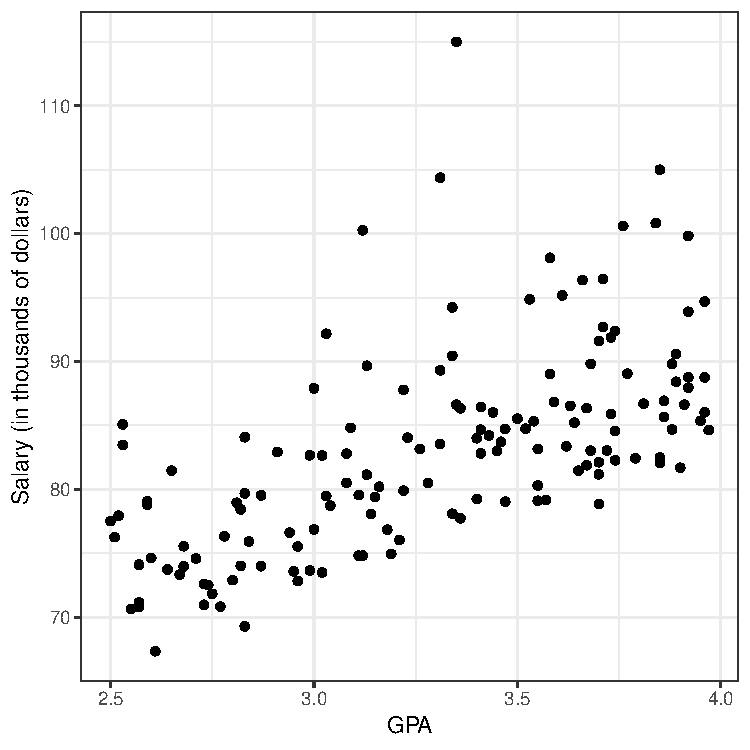
\includegraphics[width=.5\linewidth]{stat305-exam3_files/figure-latex/unnamed-chunk-3-1} 
\end{center}

Here are some summaries of the data (with GPA as \(x\) and salary as
\(y\)):

\[\sum_{i=1}^{150} x_i = 494 \hspace{3cm} \sum_{i=1}^{150} x_i^2 = 1656\]

\[\sum_{i=1}^{150} y_i = 12455 \hspace{3cm} \sum_{i=1}^{150} y_i^2 = 1043606\]

\[\sum_{i=1}^{150} x_i y_i = 41347\]

\newpage

Using the summaries above, the survey workers fit a linear relationship
between \textbf{GPA} (x) and \textbf{salary (in thousands of dollars)}
(y). \qparts{
\part[3] Write the equation of the fitted linear relationship. \vspace{5cm}
\part[3] Using the fitted linear relationship, what do we predict will be the difference in salary of an engineer with an undergraduate GPA of 3.5 and an engineer with an undergraduate GPA of 3.0? \vspace{4cm}
\part[3] The actual income of one of the surveyed engineers who had an undergraduate GPA of 3.02 was 73.5 thousand dollars. What is the residual for this specific engineer using the linear relationship? \vspace{4cm}
\part[3] For the linear relationship, find \(r\), the sample correlation coeffecient and \(R^2\), the coeffecient of determination. \vspace{3cm}
} \newpage Discouraged by the relationship between salary and GPA, the
surveyors remember that they know the address of each respondant and are
able to determine the median income of the area in which the respondant
lives. The JMP output below comes from fitting a linear relationship
using for annual salary of the respondant (``\verb!salary!'') using both
the undergraduate GPA (``\verb!GPA!'') and the median income of the area
in which the respondant lives (``\verb!med_salary_loc!'') (in thousands
of dollars).

\vspace{0.5cm}
\centerline{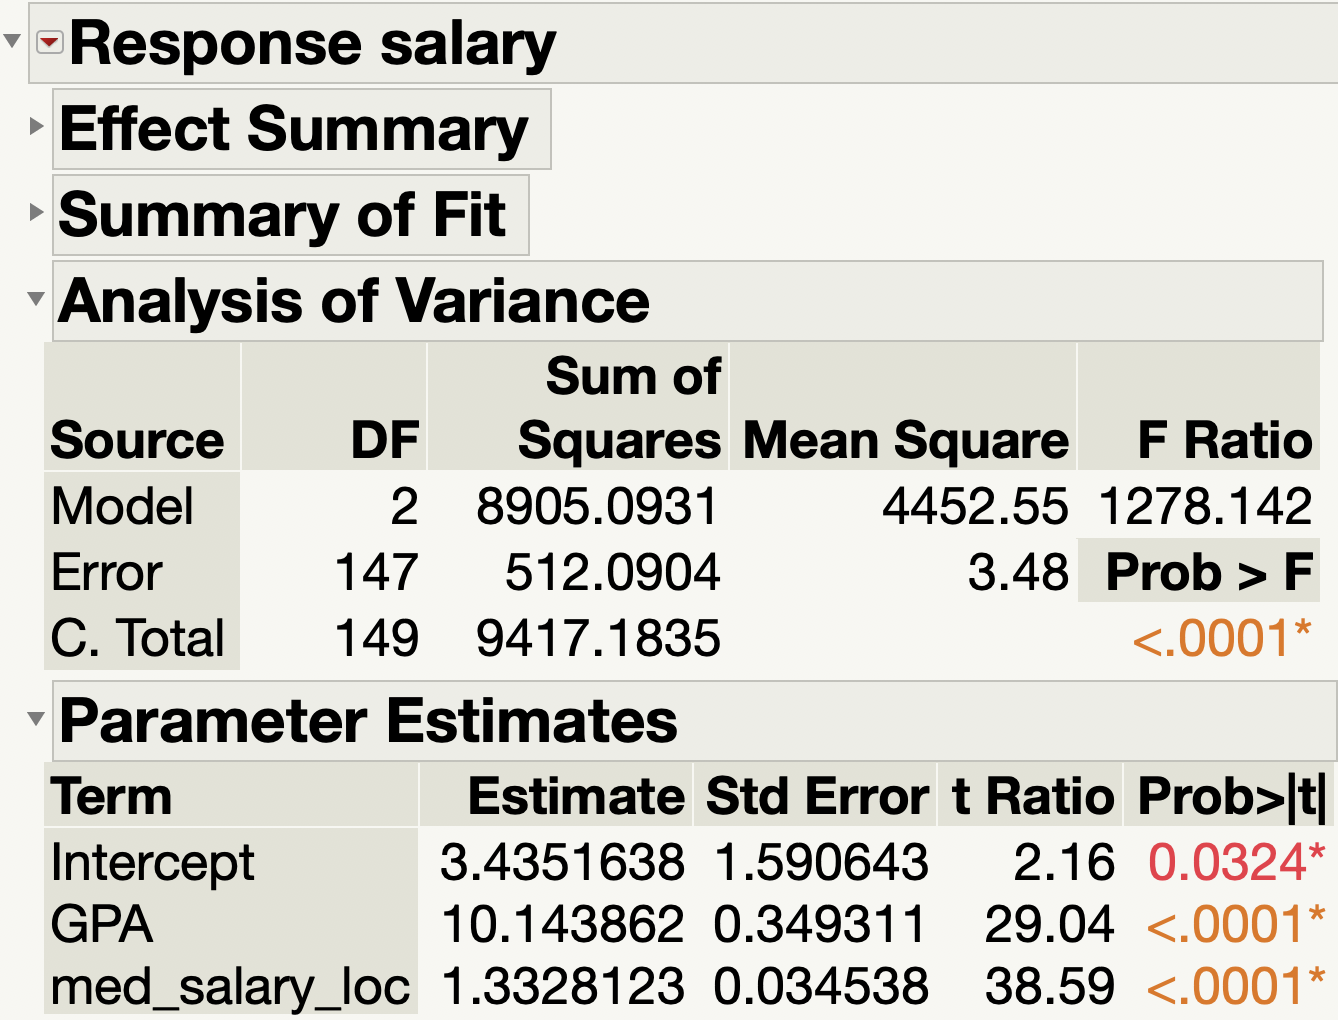
\includegraphics[scale=.4]{fit_sal}}
\vspace{0.5cm}

\qparts{
\part[3] Write the equation of this fitted multivariate linear relationship. \vspace{3cm}
\part[3] Using this fitted multivariate linear relationship, what do we suppose the salary would be for an engineer with a undergraduate GPA of 3.02 living in a location with a median income of 30.41 thousand dollars? \newpage
\part[3] The actual salary of one engineer surveyed with a undergraduate GPA of 3.02 living in a location with a median income of \$30,410 was \$73,500.  What is the residual for this specific engineer's actual salary using the fitted multivariate linear relationship? \vspace{4cm}
\part[3] Find and interpret the value of $R^2$ for the fitted multivariate linear relationship. \vspace{3cm}
\part[2] One surveyor suggested adding an interaction term for GPA and the engineer's location's median income. What practical effect would such an interaction have? \vspace{4cm}
\part[3] Does it appear that a using the median income of the engineer's location improved the fit? \vspace{2cm}
}

\newpage

\question[10]

The data reported below are the masses of 10 squirrels (in kg) found on
the campus at Iowa State University and 10 squirrels found at University
of Iowa this weekend: \% latex table generated in R 3.6.0 by xtable
1.8-4 package \% Mon May 6 14:50:05 2019

\begin{table}[ht]
\centering
\begin{tabular}{lrrrrrrrrrr}
  \hline
  & \multicolumn{10}{c}{Squirrel Number} \\
  & 1 & 2 & 3 & 4 & 5 & 6 & 7 & 8 & 9 & 10 \\
 \hline
ISU & 3.66 & 4.37 & 3.87 & 3.09 & 3.38 & 3.91 & 3.99 & 3.92 & 3.04 & 0.60 \\ 
  UI & 5.90 & 5.15 & 4.45 & 3.29 & 2.94 & 4.91 & 5.70 & 2.53 & 2.12 & 8.50 \\ 
   \hline
\end{tabular}
\end{table}

The third quartile of the Iowa State masses is 3.92 kg, the median of
the masses is 3.77 kg and the interquartile range is 0.84 kg.

The first quartile of the University of Iowa masses is 2.94 kg, the
median of the masses is 4.68 kg and the interquartile range is 2.76 kg.

\vspace{0.5cm}

Using the axes below, create a box plot for \textbf{time to failure} of
each compound.

\begin{itemize}
   \item Label the values of the boundaries of the boxes
   \item Label the values the ends of the upper and lower whiskers
   \item Draw a star over unusual observations.
\end{itemize}

\textit{For any partial credit, show all work in the additional space}
\vspace{1cm}

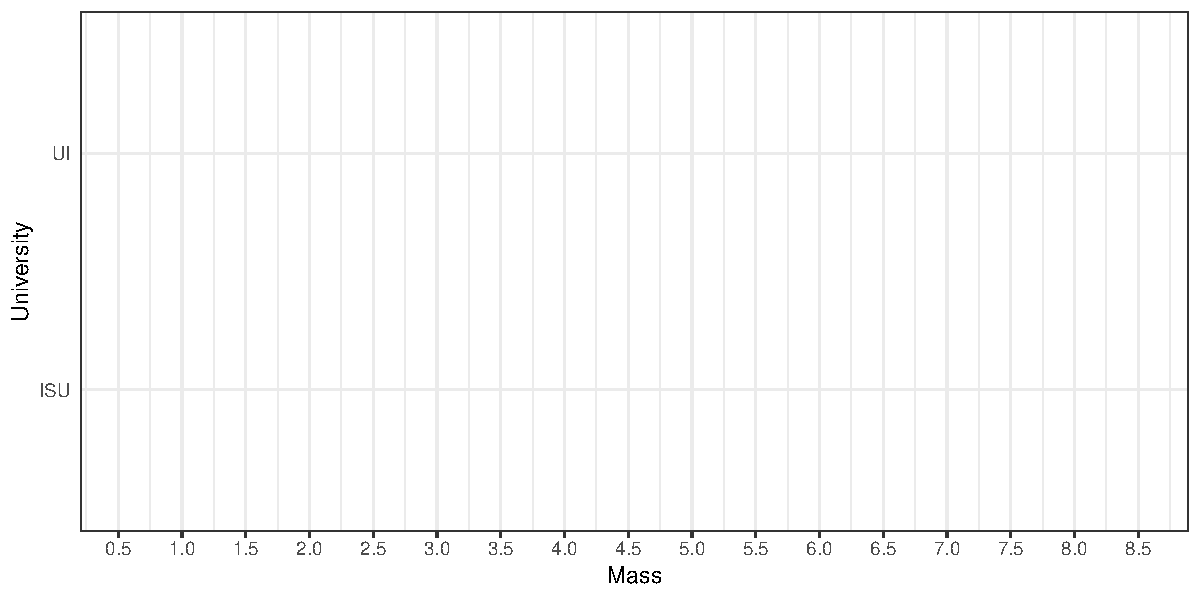
\includegraphics[width=.9\linewidth]{stat305-exam3_files/figure-latex/unnamed-chunk-4-1}

\newpage

\question

Let \(X\) be a normal random variable with a mean of -2 and a varaince
of 16 (i.e., \(X \sim N(-2, 16)\)) and let \(Z\) be a random variable
following a standard normal distribution. Find the following
probabilities (note: the attached standard normal probability table may
be helpful):

\qparts{
\part[2] $P(Z \le 1.0)$ \vspace{3cm}
\part[2] $P(|Z| \le 2.5)$ \vspace{3cm}
\part[2] $P(-8 \le X < 1)$ \vspace{4cm}
\part[3] $P(|X| \ge 4)$ \vspace{4cm}
}

\newpage

\question

Suppose that \(X\) is a discrete random variable with probability
function:
\[f(x) = \begin{cases} 0.75 (0.25)^{x-1} &  x = 1, 2, 3, \ldots \\ 0 & otherwise \end{cases}\]

\qparts{
\part[2] What is the probability that $X = 2$? \vspace{2cm}
\part[3] What is the probability that $X$ takes a value less than 4? \vspace{2cm}
\part[3] What is the probability that $X$ takes a value greater than 2? \vspace{2cm}
}

\question

The electrical grid of the tiny, struggling republic of Freedonia's
capital city depends on two independent (and sometimes functioning)
generators. Each generator is functioning approximately 75\% of the
time, allowing us to describe the number of generators operating at any
point in time, \(X\), using a binomial distribution:
\[f_X(x) = \begin{cases} \dfrac{2!}{x!(2-x)!} (0.75)^x (0.25)^{2-x} & x = 0, 1, 2 \\ 0 & otherwise \end{cases} \]
Since the generators are down so frequently, the Freedonian Power
Authority has difficulty maintaining power reserves. At any point in
time, the amount of reserve power (\(Y\), in GW) can be described using
the conditional probability:
\[P(Y \ge y | X = x) = \begin{cases} \exp\left(-\frac{y}{x+1}\right) & y \ge 0 \\ 0 & otherwise \end{cases}\]

\qparts{
\part[2] At any point in time, what is the probability that both generators are working? \newpage
\part[3] If we know that both generators are operating, what is probability that there is more than 1 GW in reserve? \vspace{4cm}
\part[3] Find the probability that at any point in time there is more than 1 GW in reserve \textit{and} 2 generators are working. \vspace{4cm}
\part[3] What is the probability that there is more than 1 GW of power in reserve at any moment? \vspace{4cm}
\part[3] Suppose we know that we have more than 1 GW in reserve. Find the probability that both generators are operational.
}

\newpage
\question

In an effort to understand smartphone use, the American Association of
Psychologists gained access to a single day's data on 625 smartphone
users. They found that the smartphone users sampled spent an average of
270 minutes using their phone on that day with a standard deviation of
phone use was 32.15 minutes. \qparts{
\part[3] Provide a 95\% confidence interval for true number of minutes smartphone users spend using thier phones on average. \vspace{4cm}
\part[3] Provide a 99\% confidence lower bound for the number of minutes smartphone users spend using thier phones on average. \vspace{4cm}
\part[5] A similar study two years ago determined that smartphone users spend an average of 4 hours per day using their phones. Perform a hypothesis test at the $\alpha = 0.05$ significance level for the claim that this is no longer the case.
}

\newpage
\question

A team of engineers is studying the differences in camera systems on
self-driving cars. Their primary concern is in the car's ability to
avoid obstacles. Each system was installed in a test car and on 10
consecutive days the car was sent on a 15 hour drive through a closed
obstacle course where the number, timing, location, and type of obstacle
the car encounters is randomly determined. The proportion of obstacles
avoided during the 15 hour drive is recorded below (along with relevant
summary statistics):

\begin{itemize}
\item System 1: 0.79, 0.87, 0.86, 0.84, 0.86, 0.87, 0.85, 0.81, 0.84, 0.78 (with $\bar{x} = 0.84, s^2 = 0.0011$)
\item System 2: 0.78, 0.77, 0.77, 0.83, 0.8, 0.81, 0.82, 0.75, 0.76, 0.75 (with $\bar{x} = 0.78, s^2 = 0.0008$)
\end{itemize}

\qparts{
\part[3] Provide a 95\% confidence interval for the mean proportion of obstacles avoided on the course using System 1. \vspace{3cm}
\part[3] Provide a 95\% confidence interval for the mean proportion of obstacles avoided on the course using System 2. \vspace{3cm}
\part[3] Assuming that the proportion of obstacles avoided is roughly normally distributed and that the both systems have the same variance in proportion of obstacles avoided, provide a 95\% confidence interval for the difference in the average proportion of obstacles avoided by two systems. \vspace{4cm} 
\part[3] Does this previous confidence interval provide any clear evidence which system is best able to avoid obstacles on the course? Explain.
}

\newpage

\question

A small military subcontractor has secured a contract to develop drones
capable of providing light air support for smaller naval vessels.
Successfully fulfilling the contract requires that the drone be able to
takeoff with a minimum runway of 10 meters. However, late changes in the
prototype's weight distribution have led to concerns that they are no
longer satisfying this requirement. Using 100 takeoffs, they found the
average distance before takeoff was 9.92 meters with a standard
deviation of 0.4 meters. \qparts{
\part[10] Conduct a hypothesis test at the $\alpha = 0.01$ significance level for $\mu$, the true average distance before takeoff with the null hypothesis $\mu \ge 10$ against the alternative hypothesis of $\mu < 10$. Include the hypothesis statement, the test statistic, the p-value, and the conclusion. \vspace{11cm}
\part[3] Does the drone prototype meet the contract's runway requirements or will they need to redesign? Explain.
}

\end{questions}

\end{document}
